\documentclass[10pt, journal, letterpaper, compsoc]{IEEEtran}
\usepackage{graphicx} % Required for inserting images
\usepackage{authblk}
\usepackage{geometry}
\usepackage{amsmath}

\usepackage{titling}
\newcommand{\subtitle}[1]{%
  \posttitle{%
    \par\end{center}
    \begin{center}\large#1\end{center}
    \vskip0.5em}%
}


\usepackage{parskip}

\def\url#1{\expandafter\string\csname #1\endcsname}

\usepackage{graphicx} %package to manage images
\graphicspath{ {images/} }
\usepackage{caption}

\usepackage[backend=biber]{biblatex}
\addbibresource{sources.bib}
\geometry{margin=1in}


\title{Demand Forecasting by use of\\Long-Short Term Memory (LSTM) Architecture}

\author{Richard Hoehn%
	\thanks{Electronic address: \texttt{rhoehn@mtmail.mtsu.edu}; corresponding author}}
\affil{Middle Tennessee State University\\ \small CSCI 7850\\ \small Prof. Dr. Joshua L. Phillips}

\date{\vspace{1em}\today}

\begin{document}


\maketitle

\begin{abstract}
This term project focused employing deep learning recurrent neural networks (RNNs) in specific the Long Short Term Memory (LSTM) architecture to predict real-world sales demand comprised of five (5) years of store sales data based on 50 different items at 10 different stores. Each data point is a single day's data-point (rows). In order to solve the this problem I employed data grouping by date and using MinMax-Scalers to normalize the data. Due to the nature of the data being from real-world sources I had to take the 7-day rolling average to smooth out the daily noise. LSTM models are frequently used\cite{pharma-sales-forecast-lstm} to analyze and make predictions based on time-series data, which is a common characteristic in demand forecasting scenarios. My LSTM model worked well using a 90-day sequence for training and validation. In order for the loss to be calculated the Mean-Squared Error (MSE) function was used with up to 150 epochs during training. Numerous plots displaying the data distributions before and after normalization plus the training vs. validation visual are presented in the results section of this paper below. With the positive results of the LSTM being able to do a "visually" good job of predicting the future demand I hypothesise that it may worth reviewing if I would get good results using individual store data to try to better predict on a individual store basis future demand.
\end{abstract}


\section{Introduction}
In this term project I focused my student learning on demand forecasting, which is the process of predicting future customer demand for products or services using a variety of data-points based on a temporal data\footnote{In this project the temporal was daily sales}.

By employing deep learning recurrent neural networks (RNNs) in specific the Long Short Term Memory (LSTM) architecture my goal was to provide a model to predict sales demand based on historical daily sales data. The LSTM model can capture complex temporal dependencies over long ranges of time and patterns in historical sales data\cite{pharma-sales-forecast-lstm, predicting-sales-lstm, lstm-gru-performance} making it\footnote{The LSTM Architecture} a very good option for demand forecasting tasks.

My motivation for the this project is two fold:

\textbf{Firstly}, a time-series problem is very interesting for me personally since I often question how one can predict the future based on past data; additionally how the future might change if the input of data is changed as scenario forecasting.

\textbf{Secondly}, a better understanding of RNNs in specific LSTM architectures will better my grasp of this field and help me learn for my future endeavors in Computation \& Data Sciences with regards to forecasting model design.

In order to complete this project I used data from Kaggle's Demand Forecasting challenge\cite{demand-forecasting-kernels-only} released in 2018. The dataset is comprised of five (5) years of store sales data based on 50 different items at 10 different stores. Each data point is on a daily basis; with this being said the training dataset is comprised of 912,500 rows in a \texttt{csv} file. 

My key aims for this project are:
\begin{itemize}
    \item Deploy the dataset in the cloud for remote extraction, process, and scrubbing for training, validation, testing, and graphical display purposes.
    \item Build, Train, and Validate the LSTM model with the processed Kaggle\cite{demand-forecasting-kernels-only} dataset.
    \item \textit{and finally}, using multiple potting techniques provide a graphical approach to reviewing the performance of the LSTM model for prediction on the Kaggle\cite{demand-forecasting-kernels-only} dataset.
\end{itemize}

\section{Background}
LSTM models have emerged as a "go-to" tool\cite{pharma-sales-forecast-lstm, predicting-sales-lstm} in the field of demand forecasting. Based on the recurrent neural network (RNN) architecture, LSTM models are frequently used\cite{pharma-sales-forecast-lstm} to analyze and make predictions based on time-series data, which is a common characteristic in demand forecasting scenarios.

Unlike traditional RNN architectures the LSTM design can regulate the forward and backwards flow of information and more importantly be able to forget non-valuable data-traits. This means that LSTMs can remember pertinent information and utilize patterns from longer\cite{predicting-sales-lstm} historical data, which is an important feature for predicting future sales demand trends that may not be linear in nature\cite{improved-sales-forecasting}.

In many of the papers reviewed\cite{pharma-sales-forecast-lstm, predicting-sales-lstm} that extensively use the LSTM architecture to work on demand forecasts, they use tabular approaches to validate the loss and accuracy of their models; I however  plan on using some plotting techniques.


\section{Methods}
\subsection{Data Preparations}
The dataset is comprised of five (5) years of store sales data based on 50 different items at 10 different stores. Each data point is a single day's data-point (rows) with this being said the dataset is comprised of 912,500 rows in a \texttt{csv} file.

With the data being a simple tab-based row-column structure I can infer the daily total sales for all stores can be represented as a vector $s$, where each element $s_i$ is the sum of sales across all stores for day $i$.

$$
s_i = \sum_{j=1}^{n} a_{ij}
$$
In this formula:
\begin{itemize}
    \item $i$ index for days
    \item $j$ index for stores
    \item $aij$ total sales of store $j$ on day $i$
    \item $si$ total sales across all stores on day $i$
\end{itemize}


\subsection{Smoothing \& Normalization of Dataset}
Based on the description from Kaggle\cite{demand-forecasting-kernels-only} of the data it's evident that it is derived from real-world sources, suggesting it's inherent noise. It is also stated in Kaggle's information that the sales data is in whole US Dollars (\$USD).
\subsubsection{Smoothing}
In order to enhance the demand forecasting capabilities of my model, I will be using a smoothing algorithm to help the model learn more easily without the daily noise. A good methodical approach was to use a 7day moving average approach.

$$
\text{MA}_i = \frac{1}{7} \sum_{k=i-6}^{i} s_k
$$
In this formula:
\begin{itemize}
    \item $MA_i$ is the 7-day moving average on day $i$
    \item $sk$ represents the sales on day $k$
    \item The summation $\sum_{k=i-6}^{i} s_k$ calculates the total sales over the 7-day period ending on day $i$ (from day $i-6$ to day $i$)
    \item The factor $\frac{1}{7}$ averages the total sales over these 7 days
\end{itemize}

\subsubsection{Normalization}
Normalization is an important preparation step when preparing sales data for training an LSTM model\cite{improved-sales-forecasting}. This process involves scaling the sales data (in USD) so that it falls within a specific range, typically between -1 and 1. The purpose of normalization is to ensure that all sales contribute equally to the learning process, preventing some sales data with larger swings (magnitudes) from overpowering the model's learning process.

The process I chose for this project was using the \texttt{MinMaxScaler()}\footnote{Python: \texttt{from sklearn.preprocessing import MinMaxScaler}}, where the minimum value of the data becomes \textsc{-1} and the maximum value becomes \textsc{1}.

$$
x_{scaled} = \frac{x-x_{min}}{x_{max}-x_{min}}
$$

this process allowed for all the data to be ready for further 

\subsection{Sequence Data}
After smoothing and normalization, I divided the data into overlapping 90-day sequences. As an example, the first sequence consists of sales data from January 1 to March 31, and then the next from January 2 to April 1, and so on. The target variable for each sequence would be the sales data following the 90-day period, which in my case is the next day's sales data.

If the target is the sales data for the next day, and you represent the sales data for a single day as $S_t$, then the target for sequence $X_i$ would be $S_{t+1}$, where $t$ is the last day in the 90-day sequence.

$$
\mathbf{X}_i = \begin{bmatrix} 
S_{t-89} \\ 
S_{t-88} \\ 
\vdots \\ 
S_t 
\end{bmatrix}
$$

And for the target variable $y_i$, which is the sales data for the day following the 90-day sequence:

$$
\mathbf{y}_i = S_{t+1}
$$

These sequence and target pairs are then split into a 80-20 split for training and validation.


\subsection{LSTM Model \& Training}
The LSTM architecture consists of a cell state and three (3) gates: the input gate, which regulates the addition of new information to the cell state; the forget gate, which controls the removal of information irrelevant to the prediction task; and the output gate, which determines what information from the cell state to use in the output.

In order for training I use the Mean Squared Error (MSE) loss, often used in regression problems\cite{improved-sales-forecasting}, is calculated as the average of the squared differences between the predicted values and the actual values. Details of the learning late of the LSTM model can me seeing in Figure \ref{fig:mse-loss} in the following section below.

$$
\text{MSE} = \frac{1}{n} \sum_{i=1}^{n} (y_i - \hat{y}_i)^2
$$


\section{Results}
The following sections will be numerical and visual representations of the work I did on this project.

\subsection{Data Preparation \& Normalization}
As discussed in the methods section the Kaggle data is very noisy on a daily basis, hence using the 7-day average the demand is much smoother.

\begin{figure}[h]
\centering
\captionsetup{justification=centering,margin=1cm}
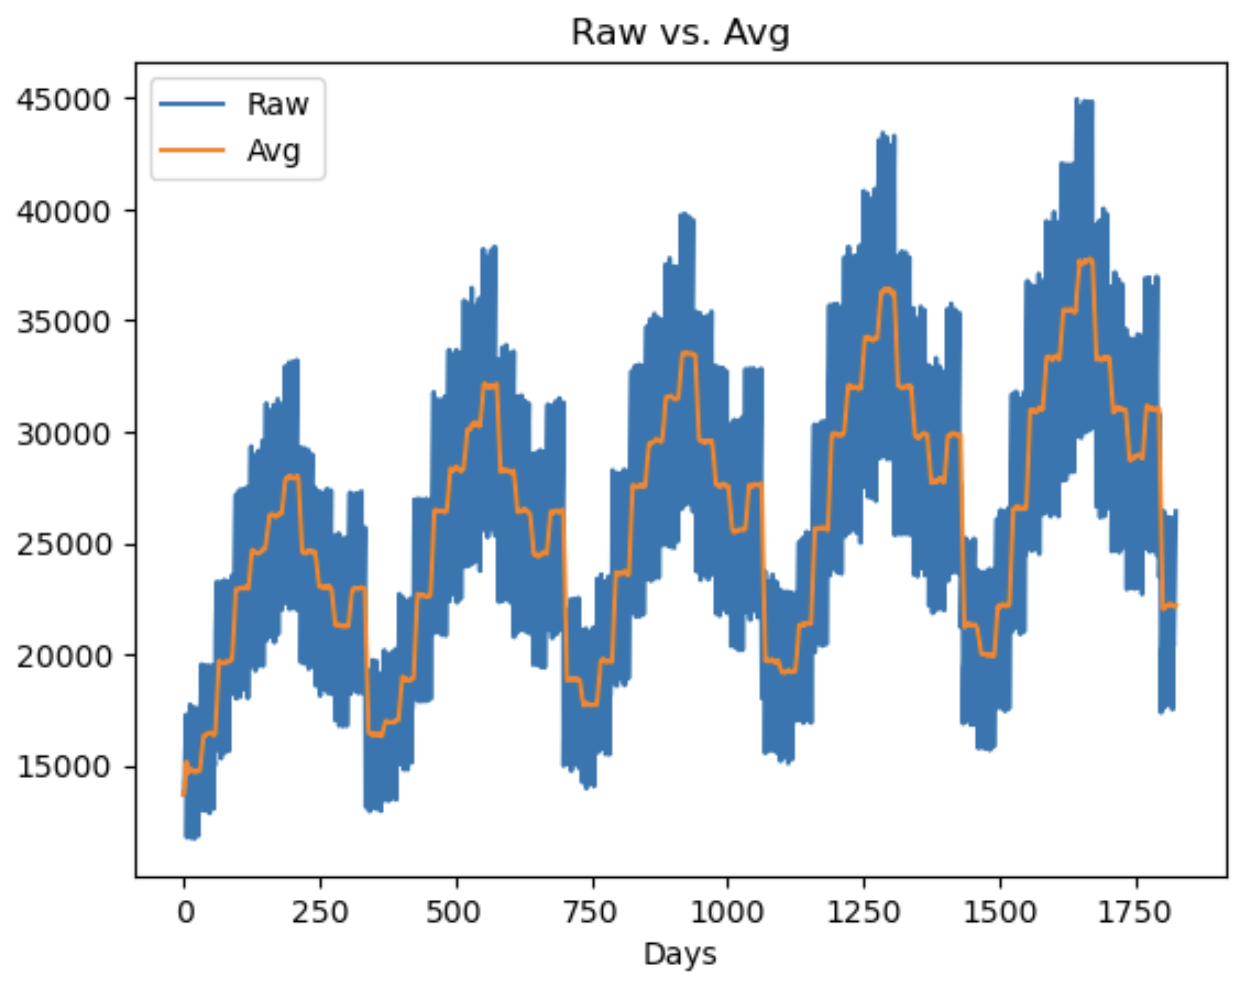
\includegraphics[width=0.45\textwidth]{raw-vs-avg.png}
\caption{Raw (Noise) Data vs. 7-Day Average}
\label{fig:raw-vs-avg}
\end{figure}

\subsection{Model Training \& Hyper-Parameter Tuning}
In table \ref{tab:hyper-parameters} one see all the used for hyper-parameters in the LSTM model setup. 

\begin{table}[h]
\centering
\begin{tabular}{|rc|rc|}
\hline
\multicolumn{4}{|c|} {LSTM Parameters} \\  
\hline
  Learning Rate  &  0.001   &  Dropout  &  0.1  \\ \hline
  Hidden Layers  &  50   &  LSTM Layers   &  4  \\ \hline
  Number of Epochs & 150 \\ \hline
\end{tabular}
\caption{Hyper-Parameter for LSTM Model}
\label{tab:hyper-parameters}
\end{table}

More table details here...

\begin{figure}[h]
\centering
\captionsetup{justification=centering,margin=1cm}
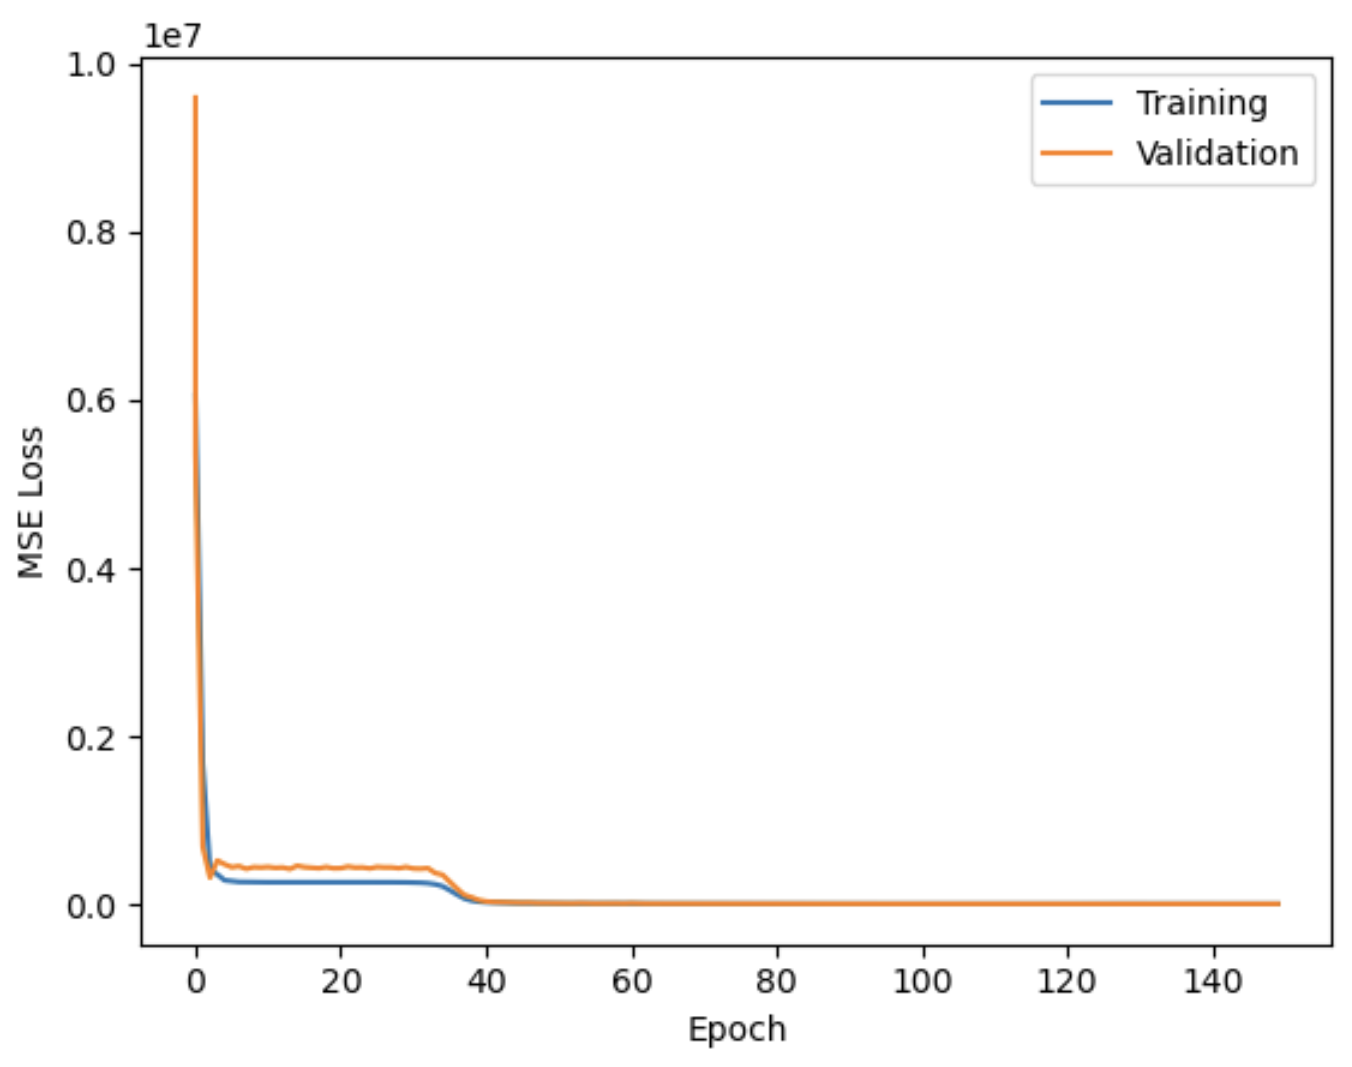
\includegraphics[width=0.45\textwidth]{mse-loss.png}
\caption{MSE Loss Details on Learning}
\label{fig:mse-loss}
\end{figure}

\subsection{Plotting of Actual and Predicted Values}
The training validation of the model are quire promising. In figure \ref{fig:true-vs-predicted} the reader can see that it overall follows the true path during the training and test phases. 

\begin{figure}[h]
\centering
\captionsetup{justification=centering,margin=1cm}
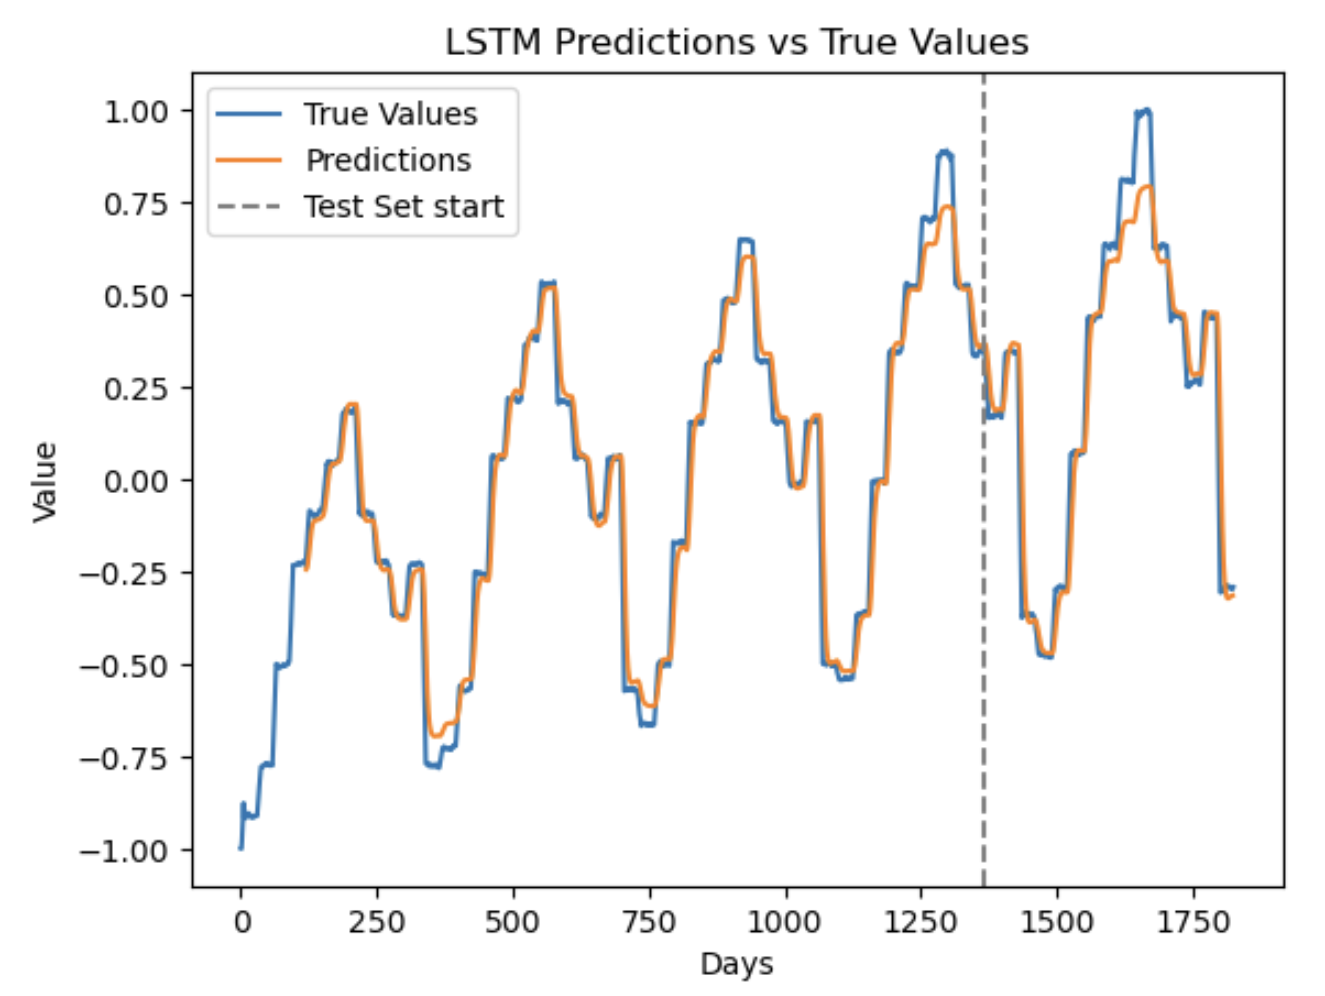
\includegraphics[width=0.45\textwidth]{true-vs-predicted.png}
\caption{True vs. Predicted during training of model}
\label{fig:true-vs-predicted}
\end{figure}



\section{Discussion}

\subsection{Review of Plots}

\subsection{Future Work}
In order to enhance the demand forecasting capabilities of my models, I intend to explore the extraction of additional contextual information related to the timestamps, such as seasons, weekdays, holidays, or any other relevant time-based factors. By incorporating these additional features into the dataset, I aim to provide the LSTM model with a richer contextual understanding of the underlying data, which can lead to more accurate predictions.

The strategy here would involve augmenting the dataset with these extracted features and subsequently comparing the performance of the LSTM models with that of the previous non-expanded dataset presented previously. This comparative analysis will shed light on the extent to which the inclusion of more temporal information influences forecasting accuracy.



\clearpage
\printbibliography %Prints bibliography
\end{document}
